\documentclass[a4paper,12pt,notitlepage]{article}
\usepackage[english]{babel}
\usepackage[a4paper, left=5mm, right=5mm, top=15mm, bottom=15mm]{geometry}
\usepackage{hyperref}
\usepackage{indentfirst}
\usepackage[utf8]{inputenc}
\usepackage{minted}
\usepackage{times}
\usepackage{inconsolata}
\usepackage[dvipsnames]{xcolor}
\linespread{1.2}

\usepackage{graphicx}
\graphicspath{{./images/}}

\definecolor{kodhatter}{HTML}{eeeeee} % minted környezetben a kód háttérszíne
\definecolor{ujpest}{HTML}{0182a2} % Hivatalos ujpest szín
\definecolor{darkujpest}{HTML}{006871} % Sötétebb nem hivatalos, jobban látszik
\definecolor{oldalhatter}{HTML}{fefbd5 } % Sötétebb nem hivatalos, jobban látszik
\pagecolor{oldalhatter}

\hypersetup{
	unicode=true, %
	colorlinks,%
	citecolor=darkujpest,%
	filecolor=darkujpest,%
	linkcolor=darkujpest,%
	urlcolor=darkujpest,%
	pdfnewwindow=true,
} %	pdftex}

%%%%%%% Fejezet stílus %%%%%%%%
\usepackage{titlesec}
\titleformat{\chapter}{\bfseries\LARGE\color{ujpest}\selectfont}{}{0pt}{{\large Chapter \thechapter.} \\  }
\titleformat{name=\chapter,numberless}{\bfseries\color{darkujpest}\selectfont}{}{0pt}{\LARGE }

\titleformat{\section}{\centering\bfseries\Large\color{ujpest}\selectfont}{}{0pt}{\thesection. \MakeUppercase }[{\titlerule[1.3pt]}]
\titleformat{name=\section,numberless}{\centering\bfseries\color{ujpest}\selectfont}{}{0pt}{\Large \MakeUppercase}[{\titlerule[1.3pt]}]

\titleformat{\subsection}{\bfseries\large\color{ujpest}\selectfont}{}{0pt}{\thesubsection. }
\titleformat{name=\subsection,numberless}{\bfseries\color{ujpest}\selectfont}{}{0pt}{\large }

\titleformat{\subsubsection}{\bfseries\itshape\color{ujpest}\selectfont}{}{0pt}{\thesubsubsection. }
\titleformat{name=\subsubsection,numberless}{\bfseries\itshape\color{ujpest}\selectfont}{}{0pt}{\itshape }
%%%%%%% Fejezet stílus %%%%%%%%

\setminted[cpp]{
    frame=lines,
    framesep=2mm,
    baselinestretch=1.2,
    bgcolor=kodhatter,
    fontsize=\footnotesize }

\begin{document}

%%%%%%%%%%%%%%%%%%%%%%%%%%%%%%%%%%%%%%%%%%%%%%%%%%%%%%%%%%%%%%%%%%%%%%%%%%%%%%%%%%%%%%%%%%%%%%%%%%%%%%

\tableofcontents

%%%%%%%%%%%%%%%%%%%%%%%%%%%%%%%%%%%%%%%%%%%%%%%%%%%%%%%%%%%%%%%%%%%%%%%%%%%%%%%%%%%%%%%%%%%%%%%%%%%%%%

\section{Creating classes}

%%%%%%%%%%%%%%%%%%%%%%%%%%%%%%%%%%%%%%%%%%%%%%%%%%%%%%%%%%%%%%%%%%%%%%%%%%%%%%%%%%%%%%%%%%%%%%%%%%%%%%

\subsection{Rule of three, five, zero}

%%%%%%%%%%%%%%%%%%%%%%%%%%%%%%%%%%%%%%%%%%%%%%%%%%%%%%%%%%%%%%%%%%%%%%%%%%%%%%%%%%%%%%%%%%%%%%%%%%%%%%

If a class requires a user-defined destructor, a user-defined copy constructor, or a user-defined
copy assignment operator, it almost certainly requires all three. Before the introduction of move
semantics in C++11, these three functions were usually referred to as the \textbf{rule of three}.
Because the presence of a user-defined (include =default or =delete declared) destructor, copy-constructor,
or copy-assignment operator prevents implicit definition of the move constructor and the move assignment
operator, any class for which move semantics are desirable, has to declare all five special member functions.
The necessity of implementing these five functions is commonly referred to as the \textbf{rule of five}.

The implicitly-defined special member functions should not be used if the class manages a resource
whose handle is an object of non-class type (raw pointer, POSIX file descriptor, etc), whose
destructor does nothing and copy constructor/assignment operator performs a "shallow copy" (copies
the value of the handle, without duplicating the underlying resource).
\href{https://en.cppreference.com/w/cpp/language/rule\_of\_three}{cppreference.com} \\
If you want a default implementation (while defining another), write =default to show you're doing
so intentionally for that function. If you don't want a generated default function, suppress it with
=delete. \\

\noindent
If you can avoid defining default operations, do. It's the simplest and gives the cleanest
semantics.\\

\noindent
When a destructor needs to be declared just to make it virtual, it can be defined as defaulted. To prevent
slicing, make the copy and move operations protected or =deleted, and add a clone. \href{https://isocpp.github.io/CppCoreGuidelines/CppCoreGuidelines#cdefop-default-operations}{C++ Core Guidelines}\\

\noindent
Writing an empty destructor can prevent the compiler from implementing certain optimizations. Use
default destructors or no destructors at all in favor of empty destructors to squeeze a little bit
more performance out of your application \cite{High_perf_cpp}.\\

\noindent
\href{https://scottmeyers.blogspot.com/2014/03/a-concern-about-rule-of-zero.html}{Scott Meyers: A Concern about the Rule of Zero}
: Classes that don't manage resources should be designed so that the compiler-generated functions
for copying, moving, and destruction do the right things. But instead of expressing this by not
declaring those functions, it's expressed by declaring them explicitly and equally explicitly opting
in to the compiler-generated implementations. With this approach, the spirit of the rule of zero
remains: classes that don't manage resources should be designed so that the compiler-generated
functions for copying, moving, and destruction do the right things. But instead of expressing this
by not declaring those functions, it's expressed by declaring them explicitly and equally explicitly
opting in to the compiler-generated implementations. The \textbf{rule of zero perhaps be the rule of the
five defaults}.

\begin{minted}{cpp}
class Widget {
public:
    Widget(const Widget&) = default;
    Widget(Widget&&) = default;
    Widget& operator=(const Widget&) = default;
    Widget& operator=(Widget&&) = default;
    // ... other constructors and functions ...
};
class CloneableBase {
public:
    virtual unique_ptr<CloneableBase> clone() const;
    virtual ~CloneableBase() = default;
    CloneableBase() = default;
    CloneableBase(const CloneableBase&) = delete;
    CloneableBase& operator=(const CloneableBase&) = delete;
    CloneableBase(CloneableBase&&) = delete;
    CloneableBase& operator=(CloneableBase&&) = delete;
    // ... other constructors and functions ...
}
\end{minted}

%%%%%%%%%%%%%%%%%%%%%%%%%%%%%%%%%%%%%%%%%%%%%%%%%%%%%%%%%%%%%%%%%%%%%%%%%%%%%%%%%%%%%%%%%%%%%%%%%%%%%%

\subsection{Destructor}

%%%%%%%%%%%%%%%%%%%%%%%%%%%%%%%%%%%%%%%%%%%%%%%%%%%%%%%%%%%%%%%%%%%%%%%%%%%%%%%%%%%%%%%%%%%%%%%%%%%%%%

\subsubsection{Virtual destructors}

\noindent
Polymorphic base classes should declare virtual destructors. If a class has any virtual functions,
it should have a virtual destructor.

\noindent
Classes not designed to be base classes or not designed to be used polymorphically should not declare
virtual destructors \cite{Meyers_eff}.

\noindent
When a destructor needs to be declared just to make it virtual, it can be defined as defaulted. To
prevent slicing, make the copy and move operations protected or =deleted, and add a clone.
\href{https://isocpp.github.io/CppCoreGuidelines/CppCoreGuidelines#cdefop-default-operationsb}{C++ Core Guidelines}

%%%%%%%%%%%%%%%%%%%%%%%%%%%%%%%%%%%%%%%%%%%%%%%%%%%%%%%%%%%%%%%%%%%%%%%%%%%%%%%%%%%%%%%%%%%%%%%%%%%%%%

\subsection{Exception in destructor}

\begin{minted}{cpp}
class Widget {
public:
    ...
    ~Widget() { ... }
};
void doSomething()
{
    std::vector<Widget> v;
    ...
}
\end{minted}

When the vector v is destroyed, it is responsible for destroying all the Widgets it contains.
Suppose v has ten Widgets in it, and during destruction of the first one, an exception is thrown.
The other nine Widgets still have to be destroyed (otherwise any resources they hold would be
leaked), so v should invoke their destructors. But suppose that during those calls, a second Widget
destructor throws an exception. Now there are two simultaneously active exceptions, and that's one
too many for C++. Depending on the precise conditions under which such pairs of simultaneously
active exceptions arise, program execution either terminates or yields undefined behavior.

Destructors should never emit exceptions. If functions called in a destructor may throw, the
destructor should catch any exceptions, then swallow them or terminate the program.

If class clients need to be able to react to exceptions thrown during an operation, the class should
provide a regular (i.e., non-destructor) function that performs the operation \cite{Meyers_eff}.

\begin{minted}{cpp}
class DBConn {
public:
    void close() // function for client use
    {
        db.close();
        closed = true;
    }
    ~DBConn()
    {
        if ( !closed ) { // close the connection if not closed
            try
            {
                db.close();
            }
            catch (...) { // if closing fails not and terminate or swallow
            ...
            }
        }
    }
private:
    DBConnection db;
    bool closed;
};
\end{minted}

%%%%%%%%%%%%%%%%%%%%%%%%%%%%%%%%%%%%%%%%%%%%%%%%%%%%%%%%%%%%%%%%%%%%%%%%%%%%%%%%%%%%%%%%%%%%%%%%%%%%%%

\subsection{Swap}

Provide a swap member function when std::swap would be inefficient for your type. Make sure your
swap doesn't throw exceptions If you offer a member swap, also offer a non-member swap that calls
the member. For classes (not templates), specialize std::swap, too. When calling swap, employ a
using declaration for std::swap, then call swap without namespace qualification \cite{Meyers_eff}.

\begin{minted}{cpp}
class Widget {
public:
    void swap( Widget& other )
    {
        using std::swap;
        swap( pImpl, other.pImpl );
    }
};
namespace std {
    template<>
    void swap<Widget>( Widget& a, Widget& b )
    {
        a.swap(b);
    }
}
\end{minted}

The "template$<>$" at the beginning of this function says that this is a total template specialization
for std::swap, and the "$<$Widget$>$" after the name of the function says that the specialization is for
when T is Widget. In other words, when the general swap template is applied to Widgets, this is the
implementation that should be used. In general, we're not permitted to alter the contents of the std
namespace, but we are allowed to totally specialize standard templates (like swap) for types of our
own creation (such as Widget). \\
Overloading function templates in STD could lead to undefined behavior. We still declare a non-member
swap that calls the member swap, we just don't declare the non-member to be a specialization or overloading
of std::swap.

\begin{minted}{cpp}
namespace WidgetStuff
{
    template<typename T>
    class Widget { ... }; // including the swap member function

    template<typename T> // non-member swap function, not part of the std namespace
    void swap( Widget<T>& a, Widget<T>& b ) {
        a.swap(b);
    }
}
\end{minted}

If any code anywhere calls swap on two Widget objects, the name lookup rules in C++ (specifically
the rules known as argument-dependent lookup or Koenig lookup) will find the Widget-specific version
in WidgetStuff.

Which swap should this call? The general one in std, which you know exists; a specialization of the
general one in std, which may or may not exist; or a T -specific one, which may or may not exist and
which may or may not be in a namespace (but should certainly not be in std)? What you desire is to
call a T -specific version if there is one, but to fall back on the general version in std if
there's not.

\begin{minted}{cpp}
template<typename T>
void doSomething( T& obj1, T& obj2 )
{
    using std::swap; // make std::swap available in this function
    ...
    swap( obj1, obj2 ); // call the best swap for objects of type T
    ...
}
\end{minted}

When compilers see the call to swap, they search for the right swap to invoke. C++'s name lookup
rules ensure that this will find any T-specific swap at global scope or in the same namespace as the
type T. (For example, if T is Widget in the namespace WidgetStuff, compilers will use
argument-dependent lookup to find swap in WidgetStuff.) If no T-specific swap exists, compilers will
use swap in std, thanks to the using declaration that makes std::swap visible in this function. Even
then, however, compilers will prefer a T-specific specialization of std::swap over the general
template, so if std::swap has been specialized for T, the specialized version will be used.

%%%%%%%%%%%%%%%%%%%%%%%%%%%%%%%%%%%%%%%%%%%%%%%%%%%%%%%%%%%%%%%%%%%%%%%%%%%%%%%%%%%%%%%%%%%%%%%%%%%%%%

\section{Object Oriented Programming}

%%%%%%%%%%%%%%%%%%%%%%%%%%%%%%%%%%%%%%%%%%%%%%%%%%%%%%%%%%%%%%%%%%%%%%%%%%%%%%%%%%%%%%%%%%%%%%%%%%%%%%

\subsection{Public inheritance}

\noindent
\textbf{Public inheritance means “is-a.”} If you write that class D (“Derived”) publicly inherits from class B (“Base”) then every object of type D is also an object of type B, but not vice versa. C++ enforces this 
interpretation of public inheritance. Consider this example. We know from everyday experience that every 
student is a person, but not every person is a student.

\begin{minted}{cpp}
class Person { ... };
class Student: public Person { ... };
\end{minted}

\noindent
Any function that expects an argument of type Person (or pointer-to-Person or reference-to-Person) will also 
take a Student object (or pointer-to-Student or reference-to-Student). This is true only for public inheritance. Everything that applies to base classes must also apply to derived classes, because every derived
class object is a base class object \cite{Meyers_eff}.

%%%%%%%%%%%%%%%%%%%%%%%%%%%%%%%%%%%%%%%%%%%%%%%%%%%%%%%%%%%%%%%%%%%%%%%%%%%%%%%%%%%%%%%%%%%%%%%%%%%%%%

\subsection{Private inheritance}

\noindent
{\bf Composition} is the relationship between types that arises when objects of one type contain objects of another type. In this example, Person objects are composed of string, Address, and PhoneNumber objects. Among programmers, the term composition has lots of synonyms. It's also known as layering, containment, aggregation, and embedding.

\begin{minted}{cpp}
class Address { ... }; // where someone lives 
class PhoneNumber { ... };
class Person {
public:
...
private:
    std::string name; // composed objects
    Address address;
    PhoneNumber voiceNumber;
    PhoneNumber faxNumber;
};
\end{minted}

Composition means either “has-a” or “is-implemented-in-terms-of.” That's because you are dealing with two different domains in your software. Some objects in your programs correspond to things in the world you are
modeling, e.g., people, vehicles, video frames, etc. Such objects are part of the application domain. Other objects are purely implementation artifacts, e.g., buffers, mutexes, search trees, etc. These kinds of
objects correspond to your software's implementation domain. When composition occurs between objects in the application domain, it expresses a has-a relationship. When it occurs in the implementation domain, it expresses an is-implemented-in-terms-of relationship.

In contrast to public inheritance, compilers will generally not convert a derived class object into a base class object if the inheritance relationship between the classes is private. That's why the call to eat fails for the object s. The second rule is that members inherited from a private base class become private members of the derived class, even if they were protected or public in the base class.

Private inheritance means is-implemented-in-terms-of. If you make a class D privately inherit from a class B, you do so because you are interested in taking advantage of some of the features available in class B, not because there is any conceptual relationship between objects of types B and D. As such, private inheritance is purely an implementation technique. Private inheritance means nothing during software design, only during software implementation.

\begin{minted}{cpp}
class Timer {
public:
    explicit Timer(int tickFrequency);
    virtual void onTick() const;
};
class Widget: private Timer {
private:
    virtual void onTick() const;
};
\end{minted}

This is a nice design, but it's worth noting that private inheritance isn't strictly necessary. If we were determined to use composition instead, we could. We'd just declare a private nested class inside Widget that would publicly inherit from Timer, redefine onTick there, and put an object of that type inside Widget.

\begin{minted}{cpp}
class Widget {
private:
    class WidgetTimer: public Timer {
    public:
        virtual void onTick() const;
    };
    WidgetTimer timer;
};
\end{minted}

You might want to design Widget to allow for derived classes, but you might also want to prevent derived classes from redefining onTick. If Widget inherits from Timer, that's not possible, not even if the inheritance is private. But if WidgetTimer is private in Widget and inherits from Timer, Widget's
derived classes have no access to WidgetTimer, hence can't inherit from it or redefine its virtual functions.

\begin{minted}{cpp}
class Empty {}; // has no data, so objects should use no memory
class HoldsAnInt { // should need only space for an int
private:
    int x;
    Empty e; // should require no memory
};
\end{minted}

Conceptually, objects of such empty classes should use no space, because there is no per-object data to be stored. However, there are technical reasons for C++ decreeing that freestanding objects must have non-zero size. With most compilers, sizeof(Empty) is 1, because C++'s edict against zero-size freestanding objects is typically satisfied by the silent insertion of a char into “empty” objects. This constraint doesn't apply
to base class parts of derived class objects, because they're not free-standing. If you inherit from Empty instead of containing an object of that type you're almost sure to find that sizeof(HoldsAnInt) == sizeof(int). This is known as the empty base optimization (EBO). In practice, “empty” classes aren't truly empty. Though they never have non-static data members, they often contain typedefs, enums, static data members, or non-virtual functions. The STL has many technically empty classes that contain useful members (usually typedefs), including the base classes unary\_function and binary\_function, from which classes for user-defined function objects typically inherit. Thanks to widespread implementation of the EBO, such inheritance rarely increases the size of the inheriting classes.

%%%%%%%%%%%%%%%%%%%%%%%%%%%%%%%%%%%%%%%%%%%%%%%%%%%%%%%%%%%%%%%%%%%%%%%%%%%%%%%%%%%%%%%%%%%%%%%%%%%%%%

\subsection{Virtual inheritance}

Virtual inheritance is a C++ technique that ensures only one copy of a base class's member variables are inherited by grandchild derived classes. Without virtual inheritance, if two classes B and C inherit from a class A, and a class D inherits from both B and C, then D will contain two copies of A's member variables: one via B, and one via C. These will be accessible independently, using scope resolution.
\href{https://en.wikipedia.org/wiki/Virtual\_inheritance}{Virtual inheritance}

Instead, if classes B and C inherit virtually from class A, then objects of class D will contain only one set of the member variables from class A. This feature is most useful for multiple inheritance, as it makes the virtual base a common subobject for the deriving class and all classes that are derived from it. This can be used to avoid the diamond problem by clarifying ambiguity over which ancestor class to use, as from the perspective of the deriving class (D in the example above) the virtual base (A) acts as though it were the direct base class of D, not a class derived indirectly through a base (B or C).

\begin{figure}[H]
    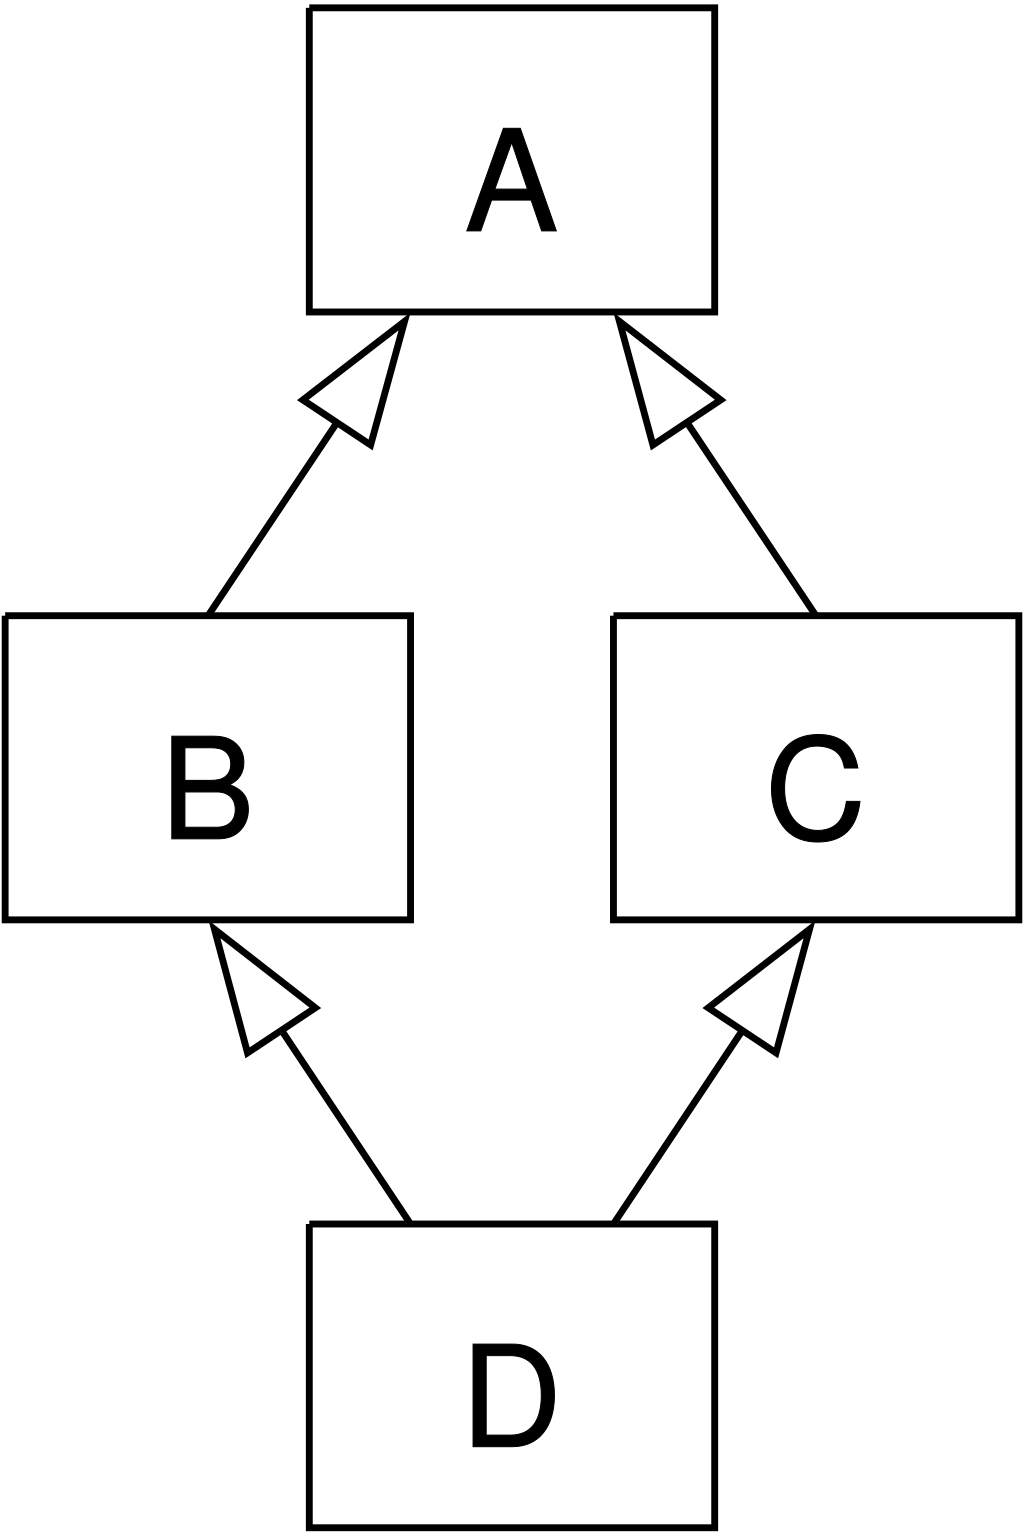
\includegraphics[width=44mm]{Diamond_inheritance.png}
    \hspace{30mm}
    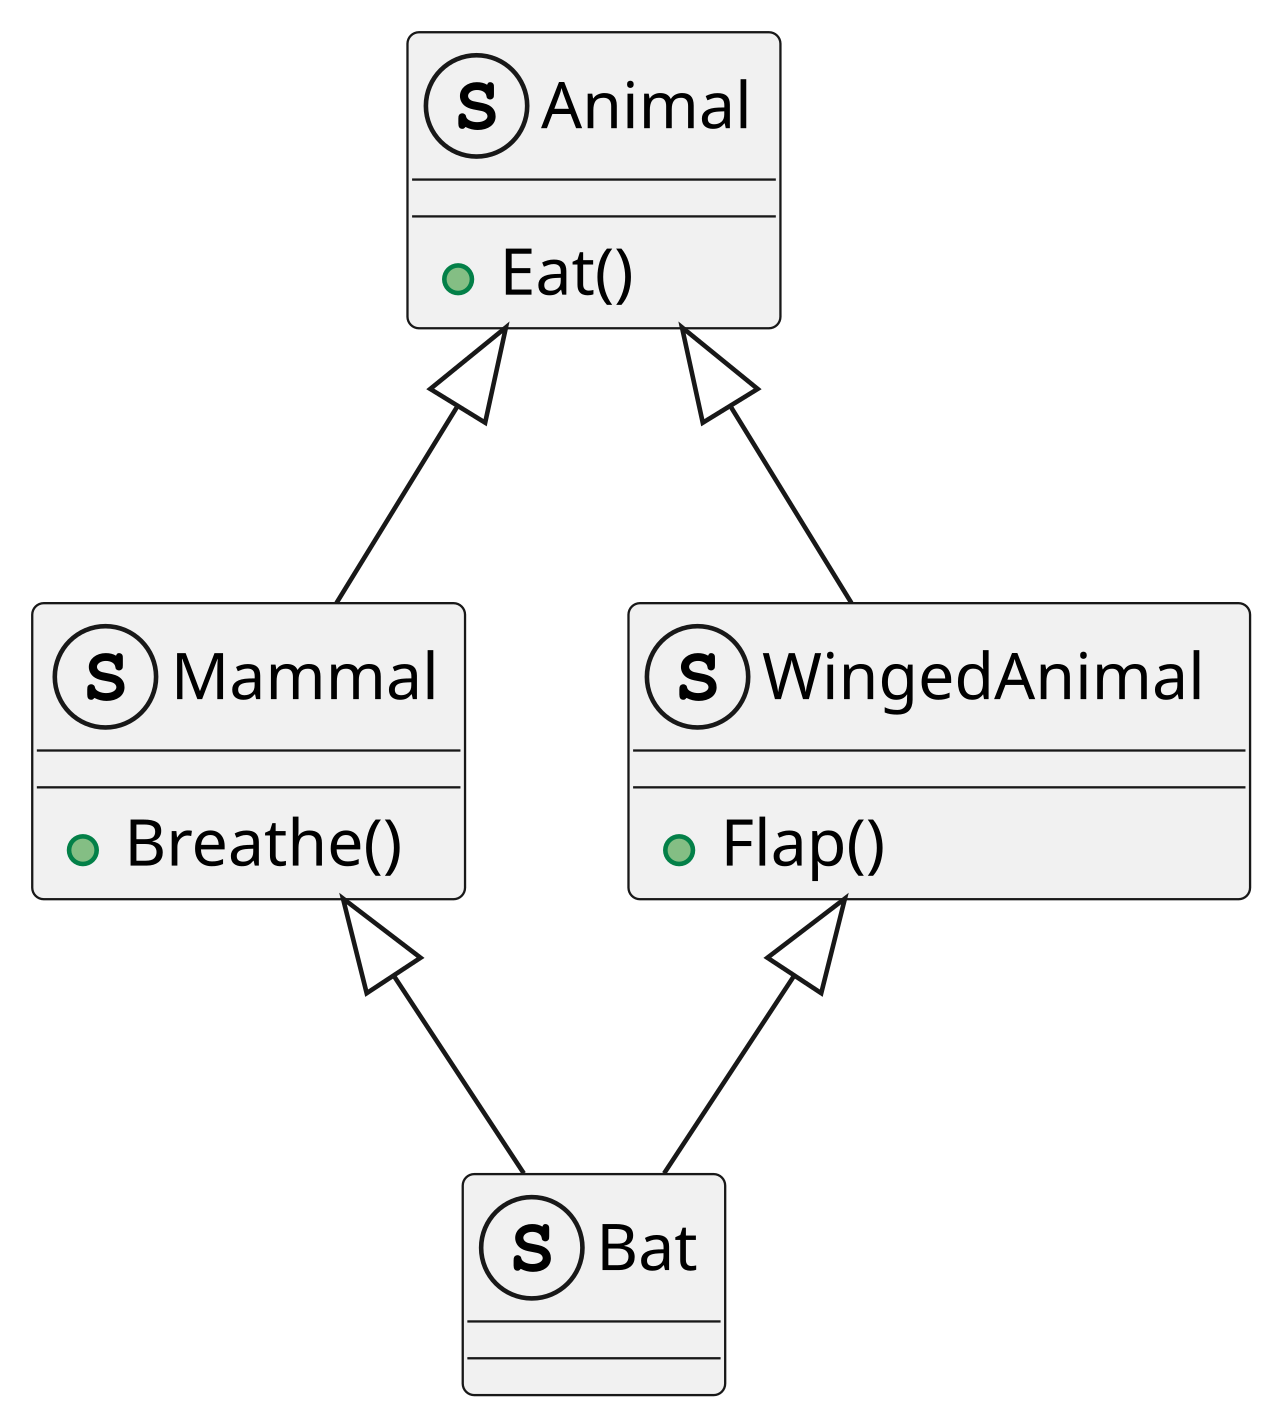
\includegraphics[width=60mm]{UML_virtual_inheritance.png}
    \centering
\end{figure}

\begin{minted}{cpp}
struct Animal {
    virtual ~Animal() = default;    // Explicitly show that the default class destructor will be made.
    virtual void Eat() {}
};
struct Mammal: Animal {
    virtual void Breathe() {}
};
struct WingedAnimal: Animal {
    virtual void Flap() {}
};
struct Bat: Mammal, WingedAnimal {}; // A bat is a winged mammal
\end{minted}

As declared above, a call to bat.Eat is ambiguous because there are two Animal (indirect) base classes in Bat, so any Bat object has two different Animal base class subobjects. So, an attempt to directly bind a reference to the Animal subobject of a Bat object would fail, since the binding is inherently ambiguous.

\begin{minted}{cpp}
Bat bat;
Animal& animal = bat;  // error: which Animal subobject should a Bat cast into?
Animal& mammal = static_cast<Mammal&>(bat); 
Animal& winged = static_cast<WingedAnimal&>(bat);
static_cast<Mammal&>(bat).Eat();
bat.Mammal::Eat();
\end{minted}

The Animal portion of Bat::WingedAnimal is now the same Animal instance as the one used by Bat::Mammal, which is to say that a Bat has only one, shared, Animal instance in its representation and so a call to Bat::Eat is unambiguous. Additionally, a direct cast from Bat to Animal is also unambiguous, now that there exists only one Animal instance which Bat could be converted to.

\begin{minted}{cpp}
struct Animal {
    virtual ~Animal() = default;
    virtual void Eat() {}
};
// Two classes virtually inheriting Animal:
struct Mammal: virtual Animal {
    virtual void Breathe() {}
};
struct WingedAnimal: virtual Animal {
    virtual void Flap() {}
};
struct Bat: Mammal, WingedAnimal {}; // A bat is still a winged mammal
\end{minted}

The ability to share a single instance of the Animal parent between Mammal and WingedAnimal is enabled by recording the memory offset between the Mammal or WingedAnimal members and those of the base Animal within the derived class. However this offset can in the general case only be known at runtime, thus Bat must become (vpointer, Mammal, vpointer, WingedAnimal, Bat, Animal). There are two vtable pointers, one per inheritance hierarchy that virtually inherits Animal. In this example, one for Mammal and one for WingedAnimal. The object size has therefore increased by two pointers, but now there is only one Animal and no ambiguity. All objects of type Bat will use the same vpointers, but each Bat object will contain its own unique Animal object. If another class inherits from Mammal, such as Squirrel, then the vpointer in the Mammal part of Squirrel will generally be different to the vpointer in the Mammal part of Bat though they may happen to be the same if the Squirrel class is the same size as Bat. 

\begin{minted}{cpp}
#include <string>
#include <iostream>

class A { 
    private: 
        std::string _msg; 
    public:
        A(std::string x): _msg(x) {} 
        void test(){ std::cout<<"hello from A: "<<_msg <<"\n"; } 
}; 

// B,C inherit A virtually
class B: virtual public A   { public: B():A("b"){}  }; 
class C: virtual public A   { public: C():A("c"){}  }; 

// since B,C inherit A virtually, A must be constructed in each child
// B() and C() constructors can be omitted
class D: public         B,C { public: D():A("d_a"),B(),C(){}  }; 
// D() constructor omitted
class E: public         D   { public: E():A("e_a"){}  }; 

// breaks without constructing A
// class D: public      B,C { public: D():B(),C(){}  }; 

// breaks without constructing A
//class E: public       D   { public: E():D(){}  }; 

int main(){
    D d; 
    d.test(); // prints: "hello from A: d_a" 
    
    E e; 
    e.test(); // prints: "hello from A: e_a"
}
\end{minted}

This example to illustrates a case where base class A has a constructor variable msg and an additional ancestor E is derived from grandchild class D. Here, A must be constructed in both D and E. Further, inspection of the variable msg illustrates how class A becomes a direct base class of its deriving class, as opposed to a base class of any intermediate deriving classed between A and the final deriving class. 

Suppose a pure virtual method is defined in the base class. If a deriving class inherits the base class virtually, then the pure virtual method does not need to be defined in that deriving class. However, if the deriving class does not inherit the base class virtually, then all virtual methods must be defined. 

\begin{minted}{cpp}
#include <string>
#include <iostream>

class A                     { 
    protected: 
        std::string _msg; 
    public:
        A(std::string x): _msg(x) {} 
        void test(){ std::cout<<"hello from A: "<<_msg <<"\n"; } 
        virtual void pure_virtual_test() = 0;
}; 

// since B,C inherit A virtually, the pure virtual method pure_virtual_test doesn't need to be defined
class B: virtual public A   { public: B(std::string x):A("b"){}  }; 
class C: virtual public A   { public: C(std::string x):A("c"){}  }; 

// since B,C inherit A virtually, A must be constructed in each child
// however, since D does not inherit B,C virtually, the pure virtual method in A must be defined
class D: public B,C { 
    public: 
        D(std::string x):A("d_a"),B("d_b"),C("d_c"){}
        void pure_virtual_test() override { std::cout<<"pure virtual hello from: "<<_msg <<"\n"; }
}; 

// it is not necessary to redefine the pure virtual method after the parent defines it
class E: public D { 
    public: 
    E(std::string x):A("e_a"),D("e_d"){}  
};

int main(){
    D d("d");
    d.test(); // hello from A: d_a
    d.pure_virtual_test(); // pure virtual hello from: d_a

    E e("e"); 
    e.test(); // hello from A: e_a
    e.pure_virtual_test(); // pure virtual hello from: e_a
}
\end{minted}

%%%%%%%%%%%%%%%%%%%%%%%%%%%%%%%%%%%%%%%%%%%%%%%%%%%%%%%%%%%%%%%%%%%%%%%%%%%%%%%%%%%%%%%%%%%%%%%%%%%%%%

\subsection{Avoid hiding inherited names}

Names in derived classes hide names in base classes. Under public
inheritance, this is never desirable. To make hidden names visible again, employ using declarations or
forwarding functions.

All functions named mf1 and mf3 in the base class are hidden by the functions named mf1 and mf3 in the derived class. This means that if you inherit from a base class with overloaded functions and you want to redefine or override only some of them, you need to include a using declaration for each name you'd otherwise be hiding. If you don't, some of the names you'd like to inherit will be hidden \cite{Meyers_eff}.

\begin{minted}{cpp}
class Base {
private:
    int x;
public:
    virtual void mf1() = 0;
    virtual void mf1(int);
    virtual void mf2();
    void mf3();
    void mf3(double);
...
};
class Derived: public Base {
public:
    using Base::mf1; // make all things in Base named mf1 and mf3 visible (and public) in Derived’s scope
    using Base::mf3;
    virtual void mf1();
    void mf3();
    void mf4();
...
};
\end{minted}

It's conceivable that you sometimes won't want to inherit all the functions from your base classes. Under public inheritance, this should never be the case, because, again, it violates public inheritance's is-a
relationship between base and derived classes. (That's why the using declarations above are in the public part of the derived class: names that are public in a base class should also be public in a publicly
derived class.) Under private inheritance, however, it can make sense. For example, suppose Derived privately inherits from Base, and the only version of mf1 that Derived wants to inherit is the one taking no parameters. A using declaration won't do the trick here, because a using declaration makes all inherited functions with a given name visible in the derived class. No, this is a case for a different technique, namely, a simple forwarding function.

\begin{minted}{cpp}
class Base {
public:
    virtual void mf1() = 0;
    virtual void mf1(int);
...
};
class Derived: private Base {
public:
    virtual void mf1() { Base::mf1(); } // forwarding function; implicitly inline
...
};
...
Derived d;
int x;
d.mf1(); // fine, calls Derived::mf1
d.mf1(x); // error! Base::mf1() is hidden
\end{minted}

%%%%%%%%%%%%%%%%%%%%%%%%%%%%%%%%%%%%%%%%%%%%%%%%%%%%%%%%%%%%%%%%%%%%%%%%%%%%%%%%%%%%%%%%%%%%%%%%%%%%%%

\subsection{Inheritance of interface and inheritance of implementation}

\noindent
Shape is an abstract class; its pure virtual function draw marks it as such. As a result, clients cannot create instances of the Shape class, only of classes derived from it.

\begin{minted}{cpp}
class Shape {
public:
    virtual void draw() const = 0;
    virtual void error(const std::string& msg);
    int objectID() const;
...
};
class Rectangle: public Shape { ... };
class Ellipse: public Shape { ... };
\end{minted}

The two most salient features of pure virtual functions are that they must be redeclared by any concrete class that inherits them, and they typically have no definition in abstract classes. The purpose of declaring a pure virtual function is to have derived classes inherit a function interface only. The purpose of declaring a simple virtual function is to have derived classes inherit a function interface as well as a default implementation. The interface says that every class must support a function to be
called when an error is encountered, but each class is free to handle errors in whatever way it sees fit. It turns out that it can be dangerous to allow simple virtual functions to specify both a function interface and a default implementation.

\begin{minted}{cpp}
class Airplane {
public:
    virtual void fly(const Airport& destination) = 0;
...
protected:
    void defaultFly(const Airport& destination);
};
void Airplane::defaultFly(const Airport& destination)
{
    //default code for flying an airplane to the given destination
}
class ModelA: public Airplane {
public:
    virtual void fly(const Airport& destination)
    { defaultFly(destination); }
    ...
};
class ModelC: public Airplane {
public:
    virtual void fly(const Airport& destination);
...
};
void ModelC::fly(const Airport& destination)
{
    // code for flying a ModelC airplane to the given destination
}
\end{minted}

It's also important that Airplane::defaultFly is a non-virtual function. This is because no derived class should redefine this function.

\begin{minted}{cpp}
class Airplane {
public:
    virtual void fly(const Airport& destination) = 0;
...
};
void Airplane::fly(const Airport& destination) // an implementation of a pure virtual function
{
    // default code for flying an airplane to the given destination
}
class ModelA: public Airplane {
public:
    virtual void fly(const Airport& destination) { Airplane::fly(destination); }
...
};
\end{minted}

This is almost exactly the same design as before, except that the body of the pure virtual function Airplane::fly takes the place of the independent function Airplane::defaultFly. In essence, fly has been broken into its two fundamental components. Its declaration specifies its interface (which derived classes must use), while its definition specifies its default behavior (which derived classes may use, but only if they explicitly request it).

The purpose of declaring a non-virtual function is to have derived classes inherit a function interface as well as a mandatory implementation. Because a non-virtual function identifies an invariant over specialization, it should never be redefined in a derived class. The differences in declarations for pure virtual, simple virtual, and non-virtual functions allow you to specify with precision what you
want derived classes to inherit: interface only, interface and a default implementation, or interface and a mandatory implementation, respectively \cite{Meyers_eff}.

%%%%%%%%%%%%%%%%%%%%%%%%%%%%%%%%%%%%%%%%%%%%%%%%%%%%%%%%%%%%%%%%%%%%%%%%%%%%%%%%%%%%%%%%%%%%%%%%%%%%%%

\subsection{Alternate to virtual functions}

\begin{minted}{cpp}
class GameCharacter {
public:
    virtual int healthValue() const; // derived classes may redefine this
...
};
\end{minted}

\subsubsection{Non-virtual interface idiom}

\noindent
This basic design, having clients call private virtual functions indirectly through public non-virtual member functions, is known as the non-virtual interface (NVI) idiom. It's a particular manifestation of
the more general design pattern called Template Method (a pattern that, unfortunately, has nothing to do with C++ templates). I call the non-virtual function (e.g., healthValue) the virtual function's wrapper.

\begin{minted}{cpp}
class GameCharacter {
public:
    int healthValue() const // derived classes do not redefine this
    {
        // do before stuff
        int retVal = doHealthValue(); // do the real work
        // do after stuff
    return retVal;
    }
...
private:
    virtual int doHealthValue() const // derived classes may redefine this
    {
        // default algorithm for calculating character’s health
    }
};
\end{minted}

An advantage of the NVI idiom is suggested by the “do before stuff” and “do after stuff” comments in the code. Those comments identify code segments guaranteed to be called before and after the virtual
function that does the real work. This means that the wrapper ensures that before a virtual function is called, the proper context is set up, and after the call is over, the context is cleaned up. For example, the “before” stuff could include locking a mutex, making a log entry, verifying that class invariants and function preconditions are satisfied, etc. The “after” stuff could include unlocking a mutex, verifying function post conditions, reverifying class invariants, etc. There's not really any good way to do that if you let clients call virtual functions directly. The NVI idiom involves derived classes redefining private virtual functions — redefining functions they can't call. Redefining a virtual function specifies how something is to be done. Calling a virtual function specifies when it will be done. These concerns are independent. The NVI idiom allows derived classes to redefine a virtual function, thus giving them control over how functionality is implemented, but the base class reserves for itself the right to say when the function will be called. Under the NVI idiom, it's not strictly necessary that the virtual functions be private \cite{Meyers_eff}.

%%%%%%%%%%%%%%%%%%%%%%%%%%%%%%%%%%%%%%%%%%%%%%%%%%%%%%%%%%%%%%%%%%%%%%%%%%%%%%%%%%%%%%%%%%%%%%%%%%%%%%

\subsubsection{Strategy design pattern}

A more dramatic design assertion would be to say that calculating a character's health is independent of the character's type, that such calculations need not be part of the character at all. For example, we could require that each character's constructor be passed a pointer to a health calculation function, and we could call that function to do the actual calculation:

\begin{minted}{cpp}
class GameCharacter; // forward declaration

int defaultHealthCalc( const GameCharacter& gc ); // function for the default health calculation algorithm
class GameCharacter {
public:
    typedef int (*HealthCalcFunc)(const GameCharacter&);
    explicit GameCharacter( HealthCalcFunc hcf = defaultHealthCalc ): healthFunc(hcf ) {}
    int healthValue() const
    { 
        return healthFunc(*this); 
    }
...
private:
    HealthCalcFunc healthFunc;
};
\end{minted}

Different instances of the same character type can have different health calculation functions, and health calculation functions for a particular character may be changed at runtime. For example, GameCharacter might offer a member function, setHealthCalculator, that allowed replacement of the current health calculation function.

\begin{minted}{cpp}
int loseHealthQuickly(const GameCharacter&); // health calculation funcs with different behavior
int loseHealthSlowly(const GameCharacter&);

EvilBadGuy ebg1(loseHealthQuickly); // same-type characters with different health-related behavior
EvilBadGuy ebg2(loseHealthSlowly);
\end{minted}

As a general rule, the only way to resolve the need for non-member functions to have access to non-public parts of a class is to weaken the class's encapsulation. For example, the class might declare the
non-member functions to be friends, or it might offer public accessor functions for parts of its implementation it would otherwise prefer to keep hidden. Whether the advantages of using a function pointer
instead of a virtual function (e.g., the ability to have per-object health calculation functions and the ability to change such functions at runtime) offset the possible need to decrease GameCharacter's encapsulation is something you must decide on a design-by-design basis.

%%%%%%%%%%%%%%%%%%%%%%%%%%%%%%%%%%%%%%%%%%%%%%%%%%%%%%%%%%%%%%%%%%%%%%%%%%%%%%%%%%%%%%%%%%%%%%%%%%%%%%

\subsubsection{Strategy pattern with std::function}

\begin{minted}{cpp}
class GameCharacter; // as before
int defaultHealthCalc(const GameCharacter& gc); // as before

class GameCharacter {
public:
    typedef std::function<int (const GameCharacter&)> HealthCalcFunc;
    explicit GameCharacter( HealthCalcFunc hcf = defaultHealthCalc ): healthFunc( hcf ) {}
    int healthValue() const{ return healthFunc(*this); }
...
private:
    HealthCalcFunc healthFunc;
};
\end{minted}

Compared to the last design we saw (where GameCharacter held a pointer to a function), this design is almost the same. The only difference is that GameCharacter now holds a tr1::function object — a generalized pointer to a function. That target signature is “function taking a const GameCharacter\& and returning an int.” An object of this tr1::function type (i.e., of type HealthCalcFunc) may hold any callable entity compatible with the target signature.

\begin{minted}{cpp}
short calcHealth(const GameCharacter&); // health calculation function; note non-int return type

struct HealthCalculator { // class for health calculation function objects
    int operator()(const GameCharacter&) const { ... }
};
class GameLevel { // health calculation mem function; note non-int return type
public:
    float health(const GameCharacter&) const;
...
};
class EvilBadGuy: public GameCharacter { // as before
...
};
EvilBadGuy ebg1(calcHealth); // using a function
EvilBadGuy ebg2(HealthCalculator()); // using a function object
GameLevel currentLevel;
EvilBadGuy ebg3( std::bind(&GameLevel::health,currentLevel,_1) ); // using a member function 
\end{minted}

We want to say that to calculate ebg3's health rating, the health member function in the GameLevel class should be used. Now, GameLevel::health is a function that is declared to take one parameter (a reference to a GameCharacter), but it really takes two, because it also gets an implicit GameLevel parameter — the one this points to. Health calculation functions for GameCharacters, however, take a single parameter: the GameCharacter whose health is to be calculated. If we're to use GameLevel::health for eb3's health calculation, we have to somehow “adapt” it so that instead of taking two parameters (a GameCharacter and a GameLevel), it takes only one (a GameCharacter). In this example, we always want to use currentLevel as the GameLevel object for ebg2's health calculation, so we “bind” currentLevel as the GameLevel object to be used each time GameLevel::health is called to calculate ebg3's health. That's what the std::bind call does: it specifies that ebg3's health calculation function should always use currentLevel as the GameLevel object.

%%%%%%%%%%%%%%%%%%%%%%%%%%%%%%%%%%%%%%%%%%%%%%%%%%%%%%%%%%%%%%%%%%%%%%%%%%%%%%%%%%%%%%%%%%%%%%%%%%%%%%

\section{Virtual functions}

%%%%%%%%%%%%%%%%%%%%%%%%%%%%%%%%%%%%%%%%%%%%%%%%%%%%%%%%%%%%%%%%%%%%%%%%%%%%%%%%%%%%%%%%%%%%%%%%%%%%%%

\subsection{Never call virtual functions during constructions or destructions}

When creating a BuyTransaction object, BuyTransaction constructor will be called, but first, a
Transaction constructor must be called; base class parts of derived class objects are constructed
before derived class parts are. The last line of the Transaction constructor calls the virtual
function logTransaction. The version of logTransaction that’s called is the one in Transaction, not
the one in BuyTransaction — even though the type of object being created is BuyTransaction \cite{Meyers_eff}.

\begin{minted}{cpp}
class Transaction { // base class for all transactions
public:
    Transaction::Transaction() { // implementation of base calss ctor
        ...
        logTransaction(); // as final action, log this transaction
    }
    virtual void logTransaction() const = 0; // make type-dependent log entry
    ...
};
class BuyTransaction: public Transaction {
public:
    virtual void logTransaction() const; // // how to log transactions of this type
}
\end{minted}

\begin{minted}{cpp}
class Transaction {
    public:
        explicit Transaction( const std::string& logInfo ) {
            ...
            logTransaction( logInfo );
        }
        void logTransaction( const std::string& logInfo ) const; // now a non-virtual function
    };
    class BuyTransaction: public Transaction {
    public:
        BuyTransaction( parameters ): Transaction( createLogString( parameters ) ) { ... }
    private:
        static std::string createLogString( parameters );
    };
\end{minted}

%%%%%%%%%%%%%%%%%%%%%%%%%%%%%%%%%%%%%%%%%%%%%%%%%%%%%%%%%%%%%%%%%%%%%%%%%%%%%%%%%%%%%%%%%%%%%%%%%%%%%%

\subsection{Never redefine an inherited non-virtual function.}

\begin{minted}{cpp}
class B {
public:
    void mf();
};
class D: public B {
public:
    void mf(); // hides B::mf
};
D x; // x is an object of type D
B *pB = &x; // get pointer to x
D *pD = &x; // get pointer to x
pB->mf(); // calls B::mf
pD->mf(); // calls D::mf
\end{minted}

The reason for this two-faced behavior is that non-virtual functions like B::mf and D::mf are statically bound. That means that because pB is declared to be of type pointer-to-B, non-virtual functions invoked through pB will always be those defined for class B, even if pB points to an object of a class derived from B, as it does in this example. Virtual functions, on the other hand, are dynamically bound, so they don't suffer from this problem. If mf were a virtual function, a call to mf through either pB or pD would result in an invocation of D::mf, because what pB and pD really point to is an object of type D.

Moreover, derived classes would invariably redefine an inherited non-virtual function: the base
class's destructor. This would be true even for derived classes that declare no destructor, because the destructor is one of the member functions that compilers generate for you if you don't declare one yourself \cite{Meyers_eff}.

%%%%%%%%%%%%%%%%%%%%%%%%%%%%%%%%%%%%%%%%%%%%%%%%%%%%%%%%%%%%%%%%%%%%%%%%%%%%%%%%%%%%%%%%%%%%%%%%%%%%%%

\subsection{Never redefine a function's inherited default parameter value.}

There are only two kinds of functions you can inherit: virtual and non-virtual. However, it's always a mistake to redefine an inherited non-virtual function, so we can safely limit our discussion here to the situation in which you inherit a virtual function with a default parameter value \cite{Meyers_eff}.

Virtual functions are dynamically bound, but default parameter values are statically bound. Static binding is also known as early binding, and dynamic binding is also known as late binding. An object's static type is the type you declare it to have in the program text.

\begin{minted}{cpp}
class Shape {
public:
    enum ShapeColor { Red, Green, Blue };
    virtual void draw(ShapeColor color = Red) const = 0; // all shapes must offer a function to draw themselves
};
class Rectangle: public Shape {
public:
    virtual void draw(ShapeColor color = Green) const; // notice the different default parameter value - bad!
};
class Circle: public Shape {
public:
    virtual void draw(ShapeColor color) const;
};
Shape *ps; // static type = Shape*
Shape *pc = new Circle; // static type = Shape*
Shape *pr = new Rectangle; // static type = Shape*
\end{minted}

In this example, ps, pc, and pr are all declared to be of type pointer-to-Shape, so they all have that as their static type. Notice that it makes absolutely no difference what they're really pointing to, their static type is Shape* regardless.

An object's dynamic type is determined by the type of the object to which it currently refers. That is, its dynamic type indicates how it will behave. In the example above, pc's dynamic type is Circle*, and pr's
dynamic type is Rectangle*. As for ps, it doesn't really have a dynamic type, because it doesn't refer to any object (yet).

Dynamic types, as their name suggests, can change as a program runs, typically through assignments. Virtual functions are dynamically bound, meaning that the particular function called is determined by the dynamic type of the object through which it's invoked. That means you may end up invoking a virtual function defined in a derived class but using a default parameter value from a base class. The fact that ps, pc, and pr are pointers is of no consequence in this matter. Were they references, the problem would persist. The only
important things are that draw is a virtual function, and one of its default parameter values is redefined in a derived class.

\begin{minted}{cpp}
ps = pc; // ps’s dynamic type is now Circle*
ps = pr; // ps’s dynamic type is now Rectangle*
pc->draw(Shape::Red); // calls Circle::draw(Shape::Red)
pr->draw(Shape::Red); // calls Rectangle::draw(Shape::Red)
pr->draw(); // calls Rectangle::draw(Shape::Red)!
\end{minted}

If default parameter values were dynamically bound, compilers would have to come up with a way to determine the appropriate default value(s) for parameters of virtual functions at runtime, which would be slower and more complicated than the current mechanism of determining them during compilation.

One of the alternatives is the non-virtual interface idiom (NVI idiom): having a public non-virtual
function in a base class call a private virtual function that derived classes may redefine.

\begin{minted}{cpp}
class Shape {
public:
    enum ShapeColor { Red, Green, Blue };
    void draw(ShapeColor color = Red) const
    {
        doDraw(color);
    }
private:
    virtual void doDraw(ShapeColor color) const = 0;
};
class Rectangle: public Shape {
public:
...
private:
    virtual void doDraw(ShapeColor color) const;
...
};
\end{minted}

%%%%%%%%%%%%%%%%%%%%%%%%%%%%%%%%%%%%%%%%%%%%%%%%%%%%%%%%%%%%%%%%%%%%%%%%%%%%%%%%%%%%%%%%%%%%%%%%%%%%%%

\section{Operators}

%%%%%%%%%%%%%%%%%%%%%%%%%%%%%%%%%%%%%%%%%%%%%%%%%%%%%%%%%%%%%%%%%%%%%%%%%%%%%%%%%%%%%%%%%%%%%%%%%%%%%%

\subsection{Handle assignment to self in operator=}

Assignment returns a reference to its left-hand argument, and that's the convention you should
follow when you implement assignment operators for your classes, have assignment operators return a
reference to *this. An assignment to self occurs when an object is assigned to itself.

\begin{minted}{cpp}
Widget& Widget::operator=(const Widget& rhs)
{
    if ( this == &rhs ) return *this; // identity test: if a self-assignment, do nothing
    delete pb;
    pb = new Bitmap(*rhs.pb);
    return *this;
}
\end{minted}

If the “new Bitmap” expression yields an exception (either because there is insufficient memory for
the allocation or because Bitmap's copy constructor throws one), the Widget will end up holding a
pointer to a deleted Bitmap. Making operator= exception-safe typically renders it
self-assignment-safe, too. As a result, it's increasingly common to deal with issues of
self-assignment by ignoring them, focusing instead on achieving exception safety.

\begin{minted}{cpp}
Widget& Widget::operator=( const Widget& rhs )
{
    if ( this == &rhs ) return *this; // identity test: if a self-assignment, do nothing
    Bitmap *pOrig = pb; // remember original pb
    pb = new Bitmap( *rhs.pb ); // point pb to a copy of rhs’s bitmap
    delete pOrig; // delete the original pb
    return *this;
}
\end{minted}

An alternative to manually ordering statements in operator= to make sure the implementation is both
exception- and self-assignment-safe is to use the technique known as “copy and swap.”

\begin{minted}{cpp}
Widget& Widget::operator=(const Widget& rhs)
{
    Widget temp(rhs); // make a copy of rhs’s data
    swap(temp); // swap *this’s data with the copy’s
    return *this;
}
\end{minted}

%%%%%%%%%%%%%%%%%%%%%%%%%%%%%%%%%%%%%%%%%%%%%%%%%%%%%%%%%%%%%%%%%%%%%%%%%%%%%%%%%%%%%%%%%%%%%%%%%%%%%%

\section{Smart pointers}

%%%%%%%%%%%%%%%%%%%%%%%%%%%%%%%%%%%%%%%%%%%%%%%%%%%%%%%%%%%%%%%%%%%%%%%%%%%%%%%%%%%%%%%%%%%%%%%%%%%%%%

\subsection{Usage with arrays}

std::unique\_ptr<int[]> automatically calls delete[] when the pointer goes out of scope, ensuring the
memory is properly freed.

\begin{minted}{cpp}
std::unique_ptr<int[]> arr( new int[10]) ;
\end{minted}

With shared\_ptr a custom deleter must be provided. Without the custom deleter, shared\_ptr will call
delete, not delete[], leading to undefined behavior.

\begin{minted}{cpp}
std::shared_ptr<int> arr( new int[10], std::default_delete<int[]>() );
\end{minted}

With C++17, shared\_ptr can be used to manage a dynamically allocated array. This handles delete[]
automatically, elements can be accesses with arr[i].

\begin{minted}{cpp}
std::shared_ptr<int[]> arr( new int[10] );
\end{minted}

%%%%%%%%%%%%%%%%%%%%%%%%%%%%%%%%%%%%%%%%%%%%%%%%%%%%%%%%%%%%%%%%%%%%%%%%%%%%%%%%%%%%%%%%%%%%%%%%%%%%%%

\subsection{Use standalone statements}

Although we're using object-managing resources everywhere here, this call may leak resources 
\cite{Meyers_eff}.

\begin{minted}{cpp}
processWidget( std::shared_ptr<Widget>(new Widget), priority() );
\end{minted}

Before compilers can generate a call to processWidget, they have to evaluate the arguments being
passed as its parameters. C++ compilers are granted considerable latitude in determining the order
in which these things are to be done. If the call to priority yields an exception, the pointer
returned from “new Widget” will be lost, because it won't have been stored in the std::shared\_ptr we
were expecting would guard against resource leaks. The way to avoid problems like this is simple:
use a separate statement to create the Widget and store it in a smart pointer, then pass the smart
pointer to processWidget.

\begin{minted}{cpp}
auto widget = std::make_shared<Widget>();
processWidget( widget, priority() );
\end{minted}

%%%%%%%%%%%%%%%%%%%%%%%%%%%%%%%%%%%%%%%%%%%%%%%%%%%%%%%%%%%%%%%%%%%%%%%%%%%%%%%%%%%%%%%%%%%%%%%%%%%%%%

\section{Exception safety}

%%%%%%%%%%%%%%%%%%%%%%%%%%%%%%%%%%%%%%%%%%%%%%%%%%%%%%%%%%%%%%%%%%%%%%%%%%%%%%%%%%%%%%%%%%%%%%%%%%%%%%

\subsection{Exception-safe functions}

When an exception is thrown, exception-safe functions \cite{Meyers_eff}:

\begin{itemize}
\item Leak no resources. The code below fails this test, because if the “new Image(imgSrc)” expression
  yields an exception, the call to unlock never gets executed, and the mutex is held forever.

\item Don't allow data structures to become corrupted. If “new Image(imgSrc)” throws, bgImage is left
  pointing to a deleted object. In addition, imageChanges has been incremented, even though it's not
  true that a new image has been installed.
\end{itemize}

\begin{minted}{cpp}
void PrettyMenu::changeBackground(std::istream& imgSrc)
{
    lock(&mutex); // acquire mutex
    delete bgImage; // get rid of old background
    ++imageChanges; // update image change count
    bgImage = new Image(imgSrc); // install new background
    unlock(&mutex); // release mutex
}
\end{minted}

Exception-safe functions offer one of three guarantees:

\begin{itemize}
\item Functions offering the basic guarantee promise that if an exception is thrown, everything in the
  program remains in a valid state. No objects or data structures become corrupted, and all objects
  are in an internally consistent state (e.g., all class invariants are satisfied). However, the
  exact state of the program may not be predictable, the program could be in any valid state.

\item Functions offering the strong guarantee promise that if an exception is thrown, the state of the
  program is unchanged. Calls to such functions are atomic in the sense that if they succeed, they
  succeed completely, and if they fail, the program state is as if they’d never been called.

\item Functions offering the nothrow guarantee promise never to throw exceptions, because they always do
  what they promise to do. All operations on built-in types (e.g., ints, pointers, etc.) are nothrow
  (i.e., offer the nothrow guarantee). This is a critical building block of exception-safe code.
\end{itemize}

\begin{minted}{cpp}
class PrettyMenu {
...
    std::shared_ptr<Image> bgImage;
...
};
void PrettyMenu::changeBackground( std::istream& imgSrc )
{
    std::unique_lock lock(mutex);
    bgImage.reset( new Image(imgSrc) ); // replace bgImage’s internal pointer
    ++imageChanges;
}
\end{minted}

The above changes almost suffice to allow changeBackground to offer the strong exception safety
guarantee. If the Image constructor throws an exception, it’s possible that the read marker for the
input stream has been moved, and such movement would be a change in state visible to the rest of the
program. Until changeBackground addresses that issue, it offers only the basic exception safety
guarantee. There is a general design strategy that typically leads to the strong guarantee, it is
known as “copy and swap.” In principle, it’s very simple. Make a copy of the object you want to
modify, then make all needed changes to the copy. If any of the modifying operations throws an
exception, the original object remains unchanged. After all the changes have been successfully
completed, swap the modified object with the original in a non-throwing operation.

\begin{minted}{cpp}
struct PMImpl // PMImpl = “PrettyMenu Impl.”
{
    std::shared_ptr<Image> bgImage;
    int imageChanges;
};
class PrettyMenu {
...
private:
    std::mutex mtx;
    std::shared_ptr<PMImpl> pImpl;
};
void PrettyMenu::changeBackground(std::istream& imgSrc)
{
    using std::swap;
    std::unique_lock lock(mtx); // acquire the mutex
    std::shared_ptr<PMImpl> pNew( new PMImpl(*pImpl) ); // copy obj. data
    pNew->bgImage.reset( new Image(imgSrc) ); // modify the copy
    ++pNew->imageChanges;
    swap(pImpl, pNew); // swap the new data into place
}
\end{minted}

This requires making a copy of each object to be modified, which takes time and space you may be
unable or unwilling to make available. The strong guarantee is highly desirable, and you should
offer it when it's practical, but it's not practical 100\% of the time.

A function can usually offer a guarantee no stronger than the weakest guarantee of the functions it
calls. The problem is side effects. As long as functions operate only on local state (e.g., someFunc
affects only the state of the object on which it's invoked), it's relatively easy to offer the
strong guarantee. When functions have side effects on non-local data, it's much harder. If a side
effect of calling is that a database is modified, it will be hard to make someFunc strongly
exception-safe. There is, in general, no way to undo a database modification that has already been
committed; other database clients may have already seen the new state of the database.

%%%%%%%%%%%%%%%%%%%%%%%%%%%%%%%%%%%%%%%%%%%%%%%%%%%%%%%%%%%%%%%%%%%%%%%%%%%%%%%%%%%%%%%%%%%%%%%%%%%%%%

\section{Inline functions}

A function defined entirely inside a class/struct/union definition, whether it's a member function
or a non-member friend function, is implicitly an inline function unless it is attached to a named
module \cite{Meyers_eff}, \href{https://en.cppreference.com/w/cpp/language/inline}{cppreference.com}. \\

\noindent
A function declared constexpr or consteval on its first declaration is implicitly an inline function.\\

\noindent
A deleted function is implicitly an inline function: its (deleted) definition can appear in more
than one translation unit. \\

\noindent
The inline specifier, when used in a decl-specifier-seq of a variable with static storage duration (static
class member or namespace-scope variable), declares the variable to be an inline variable.\
A static data member declared constexpr on its first declaration is implicitly an inline variable.

Because the meaning of the keyword inline for functions came to mean in C++17 "multiple definitions
are permitted" rather than "inlining is preferred" since C++98, that meaning was extended to
variables.

\begin{minted}{cpp}
class Person {
public:
    int age() const { return theAge; } // an implicit inline request: age is defined in a class definition
private:
    int theAge;
};
\end{minted}

%%%%%%%%%%%%%%%%%%%%%%%%%%%%%%%%%%%%%%%%%%%%%%%%%%%%%%%%%%%%%%%%%%%%%%%%%%%%%%%%%%%%%%%%%%%%%%%%%%%%%%

\section{Templates and Generic Programming}

\subsection{Using of typename}

\noindent
When declaring a template type parameter, class and typename mean exactly the same thing \cite{Meyers_eff}.

\begin{minted}{cpp}
template<class T> class Widget; // uses "class”
template<typename T> class Widget; // uses "typename”
\end{minted}

Names in a template that are dependent on a template parameter are called dependent names. When a dependent name is nested inside a class, I call it a nested dependent name. C::const\_iterator is a nested dependent name. In fact, it's a nested dependent type name, i.e., a nested dependent name that refers to a type.
Nested dependent names can lead to parsing difficulties. For example,
suppose we made print2nd even sillier by starting it this way:

\begin{minted}{cpp}
template<typename C>
void print2nd(const C& container)
{
    C::const_iterator * x;
...
}
\end{minted}

This looks like we're declaring x as a local variable that's a pointer to a C::const\_iterator. But it looks 
that way only because we "know” that C::const\_iterator is a type. But what if C::const\_iterator weren't a 
type? What if C had a static data member that happened to be named const\_iterator, and what if x happened to 
be the name of a global variable? In that case, the code above wouldn't declare a local variable, it
would be a multiplication of C::const\_iterator by x. Until C is known, there's no way to know whether C::const\_iterator is a type or isn't, and when the template print2nd is parsed, C isn't known.
C++ has a rule to resolve this ambiguity: if the parser encounters a nested dependent name in a template, it assumes that the name is not a type unless you tell it otherwise. By default, nested dependent names are not types.

\begin{minted}{cpp}
template<typename C>
void print2nd(const C& container)
{
    if (container.size() >= 2) {
        typename C::const_iterator iter(container.begin());
        ...
    }
}
\end{minted}

\noindent
typename should be used to identify only nested dependent type names; other names shouldn't have it. For example, here's a function template that takes both a container and an iterator into that container:

\begin{minted}{cpp}
template<typename C> // typename allowed (as is “class”)
void f( const C& container, // typename not allowed
typename C::iterator iter); // typename required
\end{minted}

The exception to the “typename must precede nested dependent type names” rule is that typename must not precede nested dependent type names in a list of base classes or as a base class identifier in a member initialization list.

\begin{minted}{cpp}
template<typename T>
class Derived: public Base<T>::Nested { // base class list: typename not allowed
public:
    explicit Derived(int x): Base<T>::Nested(x) // base class identifier in init. list: typename not allowed
    {
        typename Base<T>::Nested temp; // use of nested dependent type name, required
        ...
    }
};
\end{minted}

For traits member names like value\_type, a common convention is for the typedef name to be the same as the traits member name, so such a local typedef is often defined like this:

\begin{minted}{cpp}
template<typename IterT>
void workWithIterator(IterT iter)
{
    typedef typename std::iterator_traits<IterT>::value_type value_type;
    value_type temp(*iter);
    ...
}
\end{minted}

%%%%%%%%%%%%%%%%%%%%%%%%%%%%%%%%%%%%%%%%%%%%%%%%%%%%%%%%%%%%%%%%%%%%%%%%%%%%%%%%%%%%%%%%%%%%%%%%%%%%%%

\begin{thebibliography}{9}

    \bibitem{Meyers_eff}
    Scott Meyers, \textit{Effective C++}, Third Edition: 55 Specific Ways to Improve Your Programs and Designs

    \bibitem{Meyers_more_eff}
    Scott Meyers, \textit{More Effective C++: 35 New Ways to Improve Your Programs and Designs}

    \bibitem{Meyers_eff_stl}
    Scott Meyers, \textit{Effective STL : 50 Specific Ways to Improve Your Use of the Standard Template Library}

    \bibitem{Meyers_eff_modern}
    Scott Meyers, \textit{Effective Modern C++: 42 Specific Ways to Improve Your Use of C++11 and C++14}

    \bibitem{High_perf_cpp}
    Björn Andrist, Viktor Sehr, \textit{C++ High Performance}, 2020
    
\end{thebibliography}

%%%%%%%%%%%%%%%%%%%%%%%%%%%%%%%%%%%%%%%%%%%%%%%%%%%%%%%%%%%%%%%%%%%%%%%%%%%%%%%%%%%%%%%%%%%%%%%%%%%%%%

\end{document}